\begin{problem}{Молекулы}{стандартный ввод}{стандартный вывод}{10 секунд}{256 мегабайт}

В лаборатории ведется исследование процесса деления молекул. 

Ученые в рамках эксперимента помещают одну молекулу в пробирку и наблюдают над схемой ее деления, через некоторый промежуток времени в пробирке уже несколько молекул, а у ученых на руках полная схема деления.

После эксперимента ученые берут схему и считают по ней некоторую статистику: количество молекул разных уровней. Молекула является молекулой уровня $i$ тогда, когда она породила как минимум еще $i$ поколений молекул.

Но к сожалению сама схема была утеряна, из-за стажера лаборанта, осталась лишь статистика. Помогите ученым восстановить любую схему деления молекул, которая будет соответствовать этой статистике. Гарантируется, что это возможно.

\InputFile
В первой строке теста поступает число $t$ - количество проведенных экспериментов.

Затем идет описание экспериментов, каждый эксперимент описывается в две строки:

 
В первой строке описания эксперимента поступает число $n$ - количество различных уровней молекул. 

Во второй же поступает массив $a$ длины $n$, где $a[i]$ - количество в утраченной схеме молекул уровня $i$.

В первом тесте t = 3, за каждую правильную схему к эксперименту начисляется 10 баллов. Ограничения к первому тесту:

$1 \le n \le 100$

$1 \le a[i] \le 100$


Во первом тесте t = 7, за каждую правильную схему к эксперименту начисляется 10 баллов.
Ограничения ко второму тесту:

$1 \le n \le 10^6$

$1 \le a[i] \le 10^6$

Если вы хотите набрать частичные баллы по какому-то тесту, выведете вместо схемы -1.



\OutputFile
Для каждого эксперимента выведите схему деления молекул в следующем формате:

$m$ - количество молекул в схеме

пары чисел $(u, v)$, которые представляют из себя информацию вида: молекула $u$ породила молекулу $v$.

Помните, что стартовая молекула, изначально помещенная в пробирку, обязана иметь номер 0, остальные номера молекул должны находится в диапазоне $0 < x \le m$.

Схема должна соответствовать статистике.  

\Example

\begin{example}
\exmpfile{example.01}{example.01.a}%
\end{example}

\Note
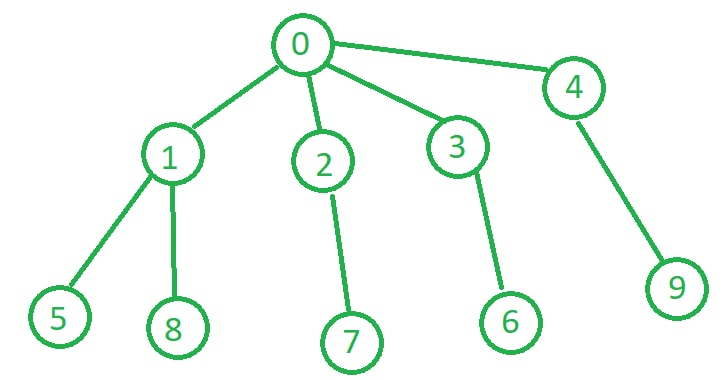
\includegraphics{example000.jpg}

Пример схемы, который мог быть у ученых на руках. 

Статистика же к этой схеме выглядит следующим образом:

$n = 3$

$a = [10, 5, 1]$

\end{problem}

